\documentclass{ExcelAtFIT}
\usepackage[T1]{fontenc}
%\documentclass[czech]{ExcelAtFIT} % when writing in CZECH
%\documentclass[slovak]{ExcelAtFIT} % when writing in SLOVAK


%--------------------------------------------------------
%--------------------------------------------------------
%	REVIEW vs. FINAL VERSION
%--------------------------------------------------------

%   LEAVE this line commented out for the REVIEW VERSIONS
%   UNCOMMENT this line to get the FINAL VERSION
%\ExcelFinalCopy


%--------------------------------------------------------
%--------------------------------------------------------
%	PDF CUSTOMIZATION
%--------------------------------------------------------

\hypersetup{
	pdftitle={Paper Title},
	pdfauthor={Jakub Fajkus},
	pdfkeywords={Keyword1, Keyword2, Keyword3}
}

%--------------------------------------------------------
%--------------------------------------------------------
%	ARTICLE INFORMATION
%--------------------------------------------------------

\ExcelYear{2018}

\PaperTitle{How to Write an Excellent Excel@FIT Paper}

\Authors{Adam Herout*}
\affiliation{*%
  \href{mailto:herout@fit.vutbr.cz}{herout@fit.vutbr.cz},
  \textit{Faculty of Information Technology, Brno University of Technology}}

\Keywords{Evolutionary computation --- Neural Networks --- Linear Genetic Programming --- Robotics}

\Supplementary{\href{http://youtu.be/S3msCdn3fNM}{Demonstration Video} --- \href{http://excel.fit.vutbr.cz/}{Downloadable Code}}


%--------------------------------------------------------
%--------------------------------------------------------
%	ABSTRACT and TEASER
%--------------------------------------------------------

\Abstract{
Tato prace se zabyva navrhem a pouzitim frameworku vyuzivajici Evolucni Algoritmy, ktery je pouzit pro hledani zpusobu rizeni pocitacoveho
modelu jednoducheho robota.
Tento robot v pocitacove simulaci vykonava pohyb po stirale tam, ze se pohybuje k danym referencnim bodum.
Pro řízení modelu robota je pouzit přístup, ktery je založeny na instrukcích, inspirovany Linearnim Genetickym Programovanim.
Program, ktery ridi robota, ma k dispozici informaci o tom, kterym smerem lezi dalsi referencni bod.
Diky informaci o smeru, kterym lezi dalsi referencni bod jsou nalezena reseni schopna pohybu i po trajektorii, na ktere nebyly uceny.
}

\Teaser{
	\TeaserImage{placeholder.pdf}
	\TeaserImage{placeholder.pdf}
	\TeaserImage{placeholder.pdf}
}



%--------------------------------------------------------
%--------------------------------------------------------
%--------------------------------------------------------
%--------------------------------------------------------
\begin{document}

\startdocument


%--------------------------------------------------------
%--------------------------------------------------------
%	ARTICLE CONTENTS
%--------------------------------------------------------

%--------------------------------------------------------
%--------------------------------------------------------
%--------------------------------------------------------
%--------------------------------------------------------
\section{Introduction}

V oblasti robotiky je velmi dulezita schopnost rychle a levne prototypovat mozna reseni.
K tomuto ucelu je velmi vhodne pouziti pocitacove modelovani a simulace.
V situaci, kdy mame navrzenou fyzickou stranku robota, nastava otazka, jak rychle prototypovat jeho rizeni.
Existuje mnoho moznosti realizace rizeni robota, lisici se v zavislosti na pozadavcich a povaze cinosti robota.
Rizeni robota muze byt zalozeno na instrukcich nejakeho imperativniho jazyka nebo na neuronovych sitich.
Dalsi z moznosti jsou ruzne planovaci algoritmy a systemy. \todo{citace, zdroje, terminologie}
Pro prototypovani je vyhodne mit nastroj, ktery je schopny hledat vyhodne zpusoby rizeni robota.
Evolutionary algorithms are good for this purpose, because they are applicable for a wide range of problems.

Hledame reseni pro problem, ktery je definovan takto.
Mame model jednoducheho robota, pro ktereho hledame model rizeni.
Cilem je nalezt program(posloupnost instrukci) ktery bude model robota ritit tak, ze bude vykonavat pohyb po dane trajektorii..
Hledani reseni probiha automatizovane s vyuzitim evolucnich algoritmu.
K vyhodnoceni uspesnosti reseni je pouzit fyzikalni simulator specializovany na simulaci robotu Mujoco\cite{Todorov2012}.

There is many works focused on evolutionary robotics.
The ones that were focusing robot control were using many techniques, including finite state machines\cite{Hodgins1996}, classical control theory\cite{Mita1984} and neural networks \cite{Reil2002}\cite{Lewis1996}.
There is also a number of works using Evolutionary Algorithms to evolve controllers, particularly artificial neural networks\cite{Randall1992}\cite{Farooq2013}.
There are also works that are using Genetic Programming\cite{Macedo2017}.
The most similar work to ours is the work of Wollf and Mattias\cite{Wolff2007}.
They are using Linear Genetic Programming to evolve a bipedal motion of a humanoid model.

Our work, as well as work of Wollf and Mattias, uses LGP with similar interpret structure.
But the program structure is a bit different.
Our approach splits the program into smaller subprograms, as opposed to one program.
Our instruction set is reduced to only one instruction and we use only natural numbers ranging from -5 to 5.
Both the works use some sort of a environmental awareness.
Our work implements that by introducing an event subprogram as well as an information about direction to the next reference point.
The subprogram is executed when an event occurs in the environment(coming closer to a reference point).
Wollf and Mattias used a set of sensors, that are measuring current joint angles of the model.

Evolved programs showed expected behaviour in the simulation.
A few best solutions were evaluated for a different trajectory and exhibited good results.
This shows that even a relatively small information about the environment and simple computational model can lead to some degree of universality of the program.

%--------------------------------------------------------
%--------------------------------------------------------
%--------------------------------------------------------
%--------------------------------------------------------
\section{Teoreticky uvod}
\label{sec:theory}
Here we will discuss a brief introduction to Linear Genetic Programming, based on \cite{Brameier2010}.
LGP is a special variant of the Genetic Programming.

Genetic Programming (GP) solves a modelling problem.
That means we know a set of inputs to a system and the outputs it should produce.
But we do not have the system that will compute the inputs and tell us the output.

In GP we are evolving computer program $P$ that represents a function: $f : I^n \to O^m$, where $I^n$ denotes the input data of $n$ dimensions and $O^m$ denotes the output data in $m$ dimensions.
When solving a control problem, we are looking for a such function, that will lead to the desired behavior.

The genotype space $G$ in GP includes all programs that can be composed of elements of a programming language $L$.
Programming language $L$ is defined by a instruction set and a terminal set.
An interpreter translates the genotype representation into the phenotype.
The phenotype is then executed and it's fitness is measured.

The original GP uses trees that correspond to expressions from a functional programming language.
The nodes of the tree represent functions, while leaves represent input values or constants.

The Linear Genetic Programming is a variant where programs are composed of a list of instructions from an imperative language or a machine code.
Each program has available predefined set of registers that can hold constants as well as results of instructions.
Those registers are often divided into groups: input registers, output registers and calculation registers.
The instructions are composed of an operation and one or more operands.
The operands may be registers or constants.
As the program is being executed it modifies the values of the registers, reads the inputs and writes the outputs.

%--------------------------------------------------------
%--------------------------------------------------------
%--------------------------------------------------------
%--------------------------------------------------------

\section{Experiments setup}
\label{sec:ExperimentsSetup}

\todo{misto fitness psat o objective function?}
V simulatoru je pripravena scena, ve ktere je umisten model robota a mnozina referencnich bodu, ktere jsou umisteny na spirale(Figure~\ref{fig:SpiralTop}) .
Robot ma za ukol se pohybovat ve scene tak, ze se ke vsem referencnim bodum priblizi co nejvice.
Timto robot vykonava pohyb po dane trajektorii.

%todo: image placement
\begin{figure}[t]
\centering
{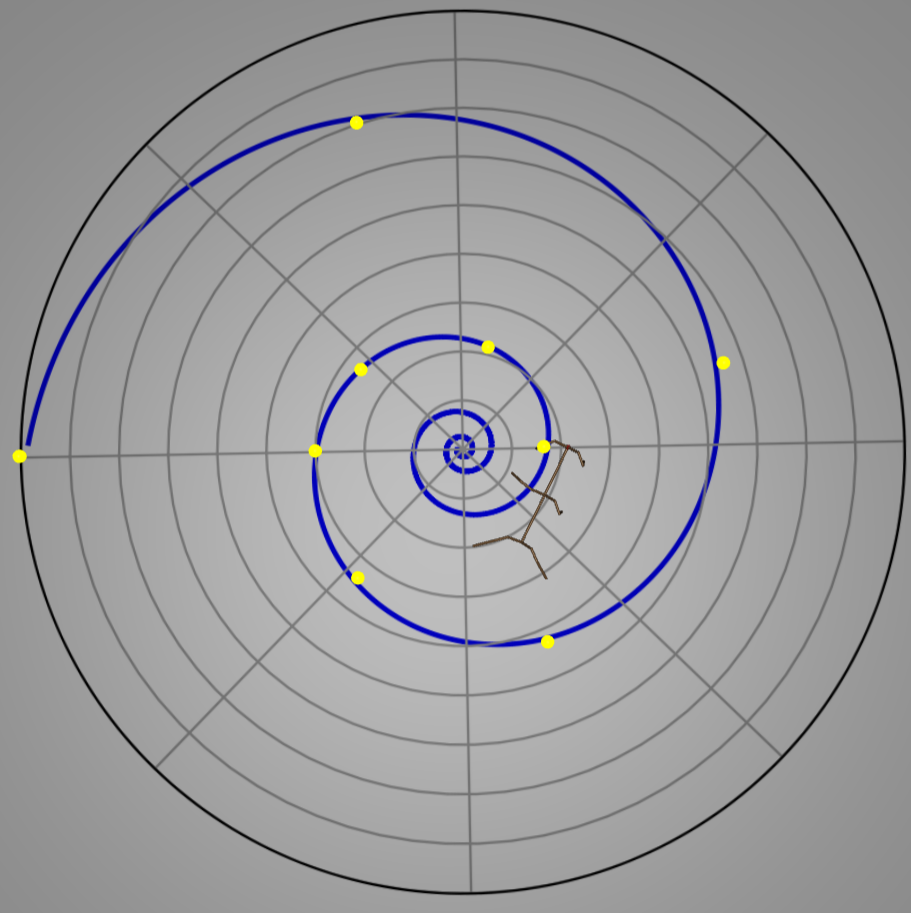
\includegraphics[height=19em]{spiral_top_v2.png}}
\caption{Top view at the scene in the simulator.
We can see a spiral on which are placed the reference points(yellow spheres).
The small brown thing is the robot model.}
\label{fig:SpiralTop}
\end{figure}


\subsection{Realizace rizeni robota}
Rizeni robota je realizovano pomoci jednoduchych instrukci.
V simulatoru je zabudovat interpret, ktery je schopny tyto instrukce prevadet na signaly, ktere zpracovava simulator.
Tyto signaly rikaji, jaka sila se bude aplikovat v jednotlivych kloubech modelu robota.
Interpret pracuje pouze s celymi cisly, a to od -5 do 5 vcetne.

Interpret obsahuje predem dany pocet vnitrnich pametovych mist(vnitrni registry), ktere je mozne modifikovat za pouziti instrukci.
Interpret take obsahuje vystupni pametova mista(vystupni registry).
Kazdy vystupni registr je prirazen k jednomu kloubu robota.
Hodnoty v techto registrech jsou prevadeny na intenzitu sily, ktera bude v techto kloubech pusobit.

Program se sklada z instrukci, ktere meni stav vnitrnich registru a stav vnejsich registru.
Tyto instrukce jsou vypsany v Table~\ref{tab:Instructions}.

Program je rozdelen do tri podprogramu - init, event a main.
Init program je proveden v nulovem case a to pouze po spusteni simulace.
Slouzi k nastaveni pocatecniho stavu vnitrnich registru. Jsou zde povoleny jen instrukce SRE a SOV\@.

Dalsim podprogramem je event.
Ten je spousten pokazde, kdyz se model robota dostatecne priblizi k nekteremu z referencnich bodu(pro kazdy bod ale pouze jednou).
Vsechny instrukce jsou provedeny v nulovem case, stejne jako v init podprogramu.
Tento podprogram slouzi ke zmene vnitrich registru.
Jsou zde povoleny instrukce SRE, SOV, INC, DEC

Hlavnim podprogramem je main.
Tento podprogram je provaden v nekonecne smycce.
Zde probiha kopirovani hodnot z vnitrnich registru do vystupnich registru.
Instrukce zde nejsou provadeny v nulovem case, ale casovy rozestup mezi nimi je 0.5 sekundy.
Jsou zde povoleny instrukce SOU, SOV.


\begin{table}[h]
	\caption{Instructions of the interpret}
	\vspace{1em}
\caption*{
INC increments an internal register by a given constant.
DEC decrements an internal register by a given constant.
SOU copies an internal register value to a output register.
SOV copies a constant value to a output register.
SRE copies a constant to an internal register.
}
	\begin{tabular}{l|{c}|r}
		\textbf{Instruction}    & \textbf{Parameter 1} & \textbf{Parameter 2}    \\
		\hline
		INC                     & Internal register    & Constant        \\
		DEC                     & Internal register    & Constant        \\
		SOU                     & Internal register    & Output register \\
		SOV                     & Constant             & Output register \\
		SRE                     & Internal register    & Constant        \\
	\end{tabular}
	\label{tab:Instructions}
\end{table}


%--------------------------------------------------------
%--------------------------------------------------------
%--------------------------------------------------------
%--------------------------------------------------------
\section{Experiements}
\label{sec:Experiments}
Zde popiseme jednitlive experimenty a nastaveni EA, ktere bylo pouzito.

\subsection{Experiment overview}
\todo{Zde bude popis experimentu - mravenec na primce? a na spirale}
\todo{Vsechny informace k experiemntu: tj. konfigurace GA, delka programu, rozdeleni na podprogramy(kolik kam), delka simulace}

\subsection{Results}
\todo{Zde budou prehledne vysledky experimentu - grafy, cisla, tabulky, obrazky, vsechno}
%--------------------------------------------------------
%--------------------------------------------------------
%--------------------------------------------------------
%--------------------------------------------------------

\section{Conclusions}
\label{sec:Conclusions}

\textbf{[Paper Summary]} What was the paper about, then? What the reader needs to remember about it?
Tato prace ukazala pouziti evolucnich algoritmu pro hledani programu pro rizeni robota. \todo{neco dalsiho}

\textbf{[Highlights of Results]} Exact numbers. Remind the reader that the paper matters.
\phony{Lorem ipsum dolor sit amet, consectetur adipiscing elit. Sed tempus fermentum ipsum at venenatis. Curabitur ultricies, mauris eu ullamcorper mattis, ligula purus dapibus mi, vel dapibus odio nulla et ex. Sed viverra cursus mattis. Suspendisse ornare semper condimentum. Interdum et malesuada fames ac ante ipsum.}

\textbf{[Paper Contributions]} What is the original contribution of this work? Two or three thoughts that one should definitely take home.
\phony{Lorem ipsum dolor sit amet, consectetur adipiscing elit. Praesent posuere mattis ante at imperdiet. Cras id tincidunt purus. Aliquam erat volutpat. Morbi non gravida nisi, non iaculis tortor. Quisque at fringilla neque.}

\textbf{[Future Work]} How can other researchers / developers make use of the results of this work?  Do you have further plans with this work? Or anybody else?
\phony{Lorem ipsum dolor sit amet, consectetur adipiscing elit. Suspendisse sollicitudin posuere massa, non convallis purus ultricies sit amet. Duis at nisl tincidunt, maximus risus a, aliquet massa. Vestibulum libero odio, condimentum ut ex non, eleifend.}

\section*{Acknowledgements}
I would like to thank my supervisor X. Y. for his help.

%--------------------------------------------------------
%--------------------------------------------------------
%--------------------------------------------------------
%	REFERENCE LIST
%--------------------------------------------------------
%--------------------------------------------------------
\phantomsection
\bibliographystyle{unsrt}
\bibliography{2018-ExcelFIT-ShortName-bib}

%--------------------------------------------------------
%--------------------------------------------------------
%--------------------------------------------------------
\end{document}
